\chapter{Theoretische Grundlagen}

Um die Qualität der Energieschätzung zu verbessern, wird ausgearbeitet, welche Anforderungen an die Analyse gestellt
werden, um zu neuen Erkenntnissen in der Astroteilchenphysik zu gelangen.
Außerdem ist ein genaues Verständnis des Random Forest Algorithmus unerlässlig, um Möglichkeiten des Qualitätsgewinns zu erarbeiten,
wobei am Ende eine sinnvolle Evaluierung der Qualität vorgenommen werden muss.

\section{Gammaastronomie}
\label{sec:Gammaastronomie}

Im Universum gibt es zahlreiche Prozesse, bei denen hochenergetische Teilchen entstehen, oder auf hohe Energien beschleunigt werden.
Bei diesen Teilchen handelt es sich zum großen Teil um Protonen oder leichte Atomkerne, aber auch Elektronen
sind Bestandteil der kosmischen Strahlung.
Ein großer Teil der Beschleunigung geschieht in Druckwellen, wie sie bei Sternexplosionen vorkommen, wobei das Modell der
Fermi-Beschleunigung erster und zweiter Ordnung eine große Rolle spielt.
%Bei der Fermi-Beschleunigung wird das Medium, indem die Druckwelle propagiert, durch ein Plasma beschrieben, welches Magnetfeldstörungen mit sich führt.
%Wenn ein geladenes Teilchen auf eine solche Störung, welche sich mit einer Geschwindigkeit $v$ durch das Medium bewegt, trifft, wird es durch die
%Lorentzkraft mit einem Winkel $\theta$ elastisch gestreut.
%Wenn nun alle möglichen Winkel berücksichtigt werden, ergibt sich eine Energiegewinn von
%\begin{equation*}
%  \left\langle \frac{\delta E}{E} \right\rangle = \frac{8}{2}\left(\frac{v}{c}\right)^2\text{ .}
%\end{equation*}
%Bei einer typischen Druckwellengeschwindigkeit von $v=\SI{e4}{\m\per\s}$~\cite[14]{HESS} ergibt sich ein Energiegewinn von $\SI{4.5e-9}{\m\per\s}$.
%Dies wird Fermibeschleunigung zweiter Art genannt und kann die große Beschleunigung in Supernovae nicht alleine erklären.
%
%Ein größeren Beitrag liefert die Fermibeschleunigung erster Art, bei der die Teilchen durch mehrfaches durchqueren der Schockfront beschleunigt werden.
%Der Energiegewinn beträgt für alle Streuwinkel
%\begin{equation*}
%  \left\langle \frac{\delta E}{E} \right\rangle \approx \frac{2}{3}\frac{\delta v}{c} \text{ ,}
%\end{equation*}
%wobei $\delta v$ der Geschwindigkeitsunterschied zwischen der Materie hinter und vor der Schockwelle ist.

Für den Teilchenfluss der kosmischen Strahlung direkt nach der Fermibeschleunigung in Schockfronten gilt
$\Phi(E)\propto E^{-2}$.
Wenn die Strahlung mit dem extragalaktischen Plasma wechselwirkt, wird das Spektrum um $E^{-\frac{1}{3}}$ steiler.
Da es auch das Plasma der Milchstraße durchqueren muss, um im Sonnensystem gemessen werden zu können, wird
der Teilchenfluss der kosmischen Strahlung durch $\Phi(E) \propto E^{-2.7}$~\cite[5]{Cosmic_rays} beschrieben.

Jedoch erklären diese Prozesse nicht den gemessenen Energiefluss von ultrahochenergetischen Teilchen, denn bei Energien von $\SI{3e15}{\eV}$ tritt ein erstes
\enquote{knee} im Spektrum auf, welches nicht durch die Fermibeschleunigung erklärt wird.
Die Phänomene, die Materie bis auf diese Energien beschleunigen, sind noch nicht vollständig erforscht.
Ein möglicher Prozess wäre die Beschleunigung durch elektrische Potentialunterschiede oder der Zerfall von Dunkler Materie.

Diese hochenergetische Teilchenstrahlung erzeugt Gammastrahlung.
Wichtige Prozesse bei der Erzeugung hochenergetischer Photonen sind die Wechselwirkungen von Photonen und Elektronen, wie
die inverse Comptonstreuung, bei der das geladene Teilchen Energie auf das Photon
überträgt. Aber auch die Annihilation, welche den Umkehrprozess der Paarerzeugung darstellt und aus einem Elektron-Positron-Paar
ein Photon-Paar erzeugt, und die Bremsstrahlung, bei der ein Photon bei der Impulsänderung geladener Teilchen abgestrahlt wird, spielen eine Rolle.
Eine weitere Möglichkeit Gammastrahlung zu erzeugen ist der Zerfall von Dunkler Materie.

\begin{figure}
  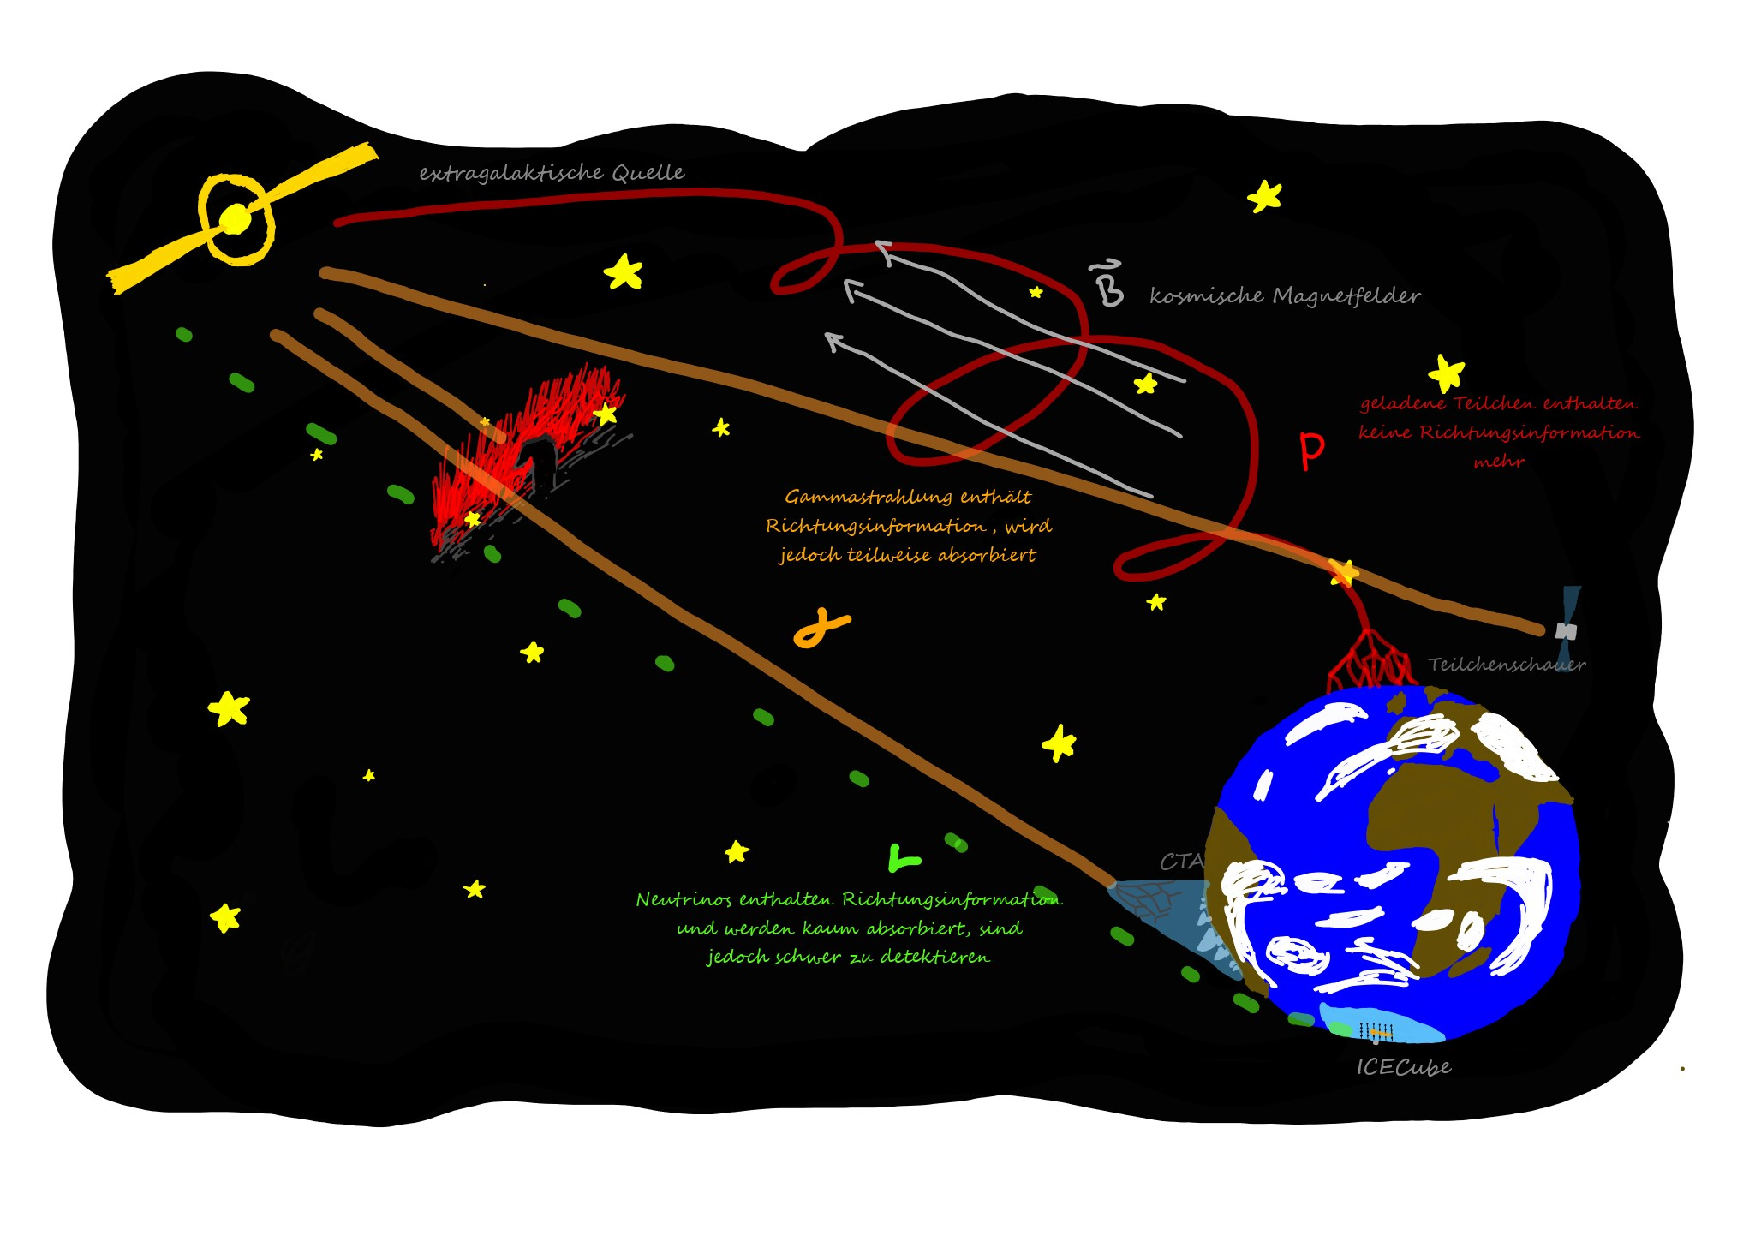
\includegraphics[width=\textwidth]{Plots/Folie5.pdf}
  \centering
  \caption{Skizzierter Weg der kosmischen Strahlung zur Erde. Die Gamma- und Neutrinostrahlung gelangt auf direktem Weg zur Erde, im Gegensatz
            zur geladenen Teilchenstrahlung, die durch kosmische Magnetfelder abgelenkt werden. Die Gammastrahlung wird durch Gaswolken teilweise
            absorbiert. Die Neutrinostrahlung ist jedoch schwer zu detektieren (angelehnt an \cite{Folie5}).}
  \label{abb:Folie5}
\end{figure}

\autoref{abb:Folie5} stellt den Weg der kosmischen Strahlung zur Erde dar, wobei die Photonen nicht mit kosmischen Magnetfeldern wechselwirken
und somit deren Ursprungsrichtung rekonstruiert werden kann. Jedoch wechselwirken die Photonen mit interstellarem Staub, der zwischen der Erde und der
Quelle ist, wodurch ein Teil der Gammastrahlung nicht zur Erde gelangt.

Diese hochenergetischen Photonen können entweder mithilfe von Satelliten im Weltraum oder mithilfe von Cherenkov-Teleskopen auf
der Erdoberfläche beobachtet werden.
Aufgrund der hohen Energien der Gammastrahlung messen Satelliten diese mithilfe von Szintillationszählern, dessen Detektionsfläche
aufgrund technischer Umsetzbarkeit begrenzt ist.
Energiereiche Strahlung sorgt jedoch dafür, dass in der Erdatmosphäre durch die Wechselwirkung mit den Luftmolekülen ein hochrelativistisches
Teilchenschauer aus überlichtschnellen geladenen Teilchen entsteht.

Da sich bei Geschwindigkeiten über der Lichtgeschwindigkeit des Mediums die durch die Polarisierung entstandenen elektromagnetischen Wellen
nicht mehr destruktiv überlagern, entstehen Cherenkov-Blitze mit einer Dauer von ca. $\SI{150}{\nano\s}$~\cite{Cherenkov_Licht}, welche sich kegelförmig
mit einem Winkel von
\begin{equation}
 \cos(\theta) = \frac{1}{n\beta}
\end{equation}
ausbreiten und von den Cherenkov-Teleskopen am Boden beobachtet werden können.
Diese Art der Beobachtung macht es möglich eine größere Fläche zu observieren, wodurch die Wahrscheinlichkeit ein hochenergetisches
Photon zu messen größer wird.
Der Winkel $\theta$ hängt von dem Brechungsindex $n$ der Luft ab, welcher von der Feuchtigkeit und Dichte der Luft abhängt und somit höhenabhängig ist.
Das kontinuierliche Spektrum der Cherenkov-Strahlung besitzt eine zur Frequenz proportionale Intensität im sichtbaren Bereich und
wird daher als bläulich wahrgenommen.
Die Kamera des Teleskops löst aus, wenn eine bestimmte Anzahl an Photonen des Schauers registriert werden.
Da sowohl hochenergetische Gammastrahlung als auch geladene Teilchenstrahlung
Schauer in der Atmosphäre erzeugen, gibt es einen Untergrund, der separiert werden muss.

\section{Cherenkov Teleskope Array (CTA)}
\label{sec:CTA}

Das geplante Cherenkov Teleskop Array wird von einer internationalen Kollaboration von 210 Instituten aus 32 Ländern~\cite{CTA_consortium} geführt
und bildet den nächsten Schritt in der Hochenergiegammaastronomie.
Mit einer Gesamtanzahl von 108 Teleskopen hat das Array, nach Simulationen zur Folge, in seinem Hauptenergiebereich eine Sensitivität von $\SI{0.1}{\percent}$
des Energieflusses des Krebsnebels, wodurch es ungefähr zehn Mal sensitiver als das HESS-Experiment ist~\cite{CTA_paper}.
Da der Teilchenfluss $\Phi$ der kosmischen Strahlung dem Potenzgesetz $\Phi \propto E^{-2.7}$~\cite[5]{Cosmic_rays} folgt,
treffen bei einer Energie $E$ von $\SI{1}{\tera\eV}$ noch $\SI{1}{\per\m\squared\per\s}$ Teilchen auf die Erdatmosphäre.
Um dennoch genug Ereignisse zu beobachten, muss eine möglichst große effektive Fläche observiert werden, weshalb der Standort in
Chile eine Fläche von $\approx \SI{4}{\kilo\m\squared}$ abdeckt~\cite{CTA_ob}.
Durch drei verschiedene Teleskopgrößen kann CTA Photonen mit Energien von $\SI{30}{\giga\eV}$ bis $\SI{300}{\tera\eV}$ detektieren,
was es ermöglicht, die verschiedenen Beschleunigungsprozesse im Universum zu untersuchen.
Zu den Arten gehören das LST (Large Sized Telescope) mit einer Spiegelgröße von $\SI{23}{\m}$, das MST (Medium Sized Telescope)
mit einer Größe von $\SI{11.5}{\m}$ oder $\SI{9.7}{\m}$ und das SST (Small-Sized Telescope), welches eine Größe von $\SI{4.3}{\m}$ oder $\SI{4.0}{\m}$
besitzt~\cite{CTA_tec}.
Die hohe Sensitivität und die niedrige Energieuntergrenze ermöglichen die Entdeckung neuer Quellen mit einer starken Rotverschiebung, die nur bei niedrigen
Energien sichtbar sind, da die höherenergetische Gammastrahlung mit dem extragalaktischen Hintergrundlicht wechselwirkt und somit nicht beobachtet werden kann.
Die große Anzahl an Teleskopen führt zusätzlich auf eine bessere Winkelauflösung, was entscheidend bei der Multiwellenlängen-Beobachtung von Quellen ist.
Diese Multiwellenlängen-Beobachtung ist entscheidend für das vollständige Verständnis der Beschleunigungsprozesse.

\section{Maschinelles Lernen}
\label{sec:ML}

Aufgrund des geringen Teilchenflusses bei hohen Energien, muss die Anzahl an beobachteten Ereignissen bei modernen
Experimenten stark ansteigen, wodurch eine händische Analyse unmöglich wird.
Daher werden Algorithmen des maschinellen Lernens trainiert, die diese Aufgabe übernehmen.
Das maschinelle Lernen wird als Teilgebiet der künstlichen Intelligenz verstanden. Hierbei lernen Algorithmen aus Datensätzen,
indem sie verschiedene Optimierungsverfahren nutzen, um eine Fehlerfunktion zu minimieren.
Ein trainierter Algorithmus kann im Anschluss Vorhersagen über neue Datenpunkte treffen.

Der Bereich des maschinellen Lernens wird in das überwachte Lernen, bei dem der Algorithmus vor einer Vorhersage mit einem Datensatz, bei dem das Ergebnis und die Eingangsdaten bekannt
sind, trainiert wird, und das unüberwachte Lernen, bei dem der Algorithmus Muster in den Eingangsdaten sucht, gegliedert.
Zwei große Aufgabengebiete im Bereich des überwachten Lernens sind die Regression und die Klassifikation. Die Regression bildet
auf die reellen Zahlen ab und die Klassifikation auf $N$ Klassen, womit die Regression als Grenzfall $N \to \infty$ der Klassifikation
verstanden werden kann.

Das Modell der Regressionsanalyse benutzt die abhängige Variable $\symbf{y}$ die über eine Funktion $f(\symbf{X},\symbf{\theta})$ von der Variable $\symbf{X}$ abhängt, um
den Parameter $\symbf{\theta}$ so zu optimieren, dass für $\symbf{\hat{y}} = f(\symbf{X},\symbf{\theta}) + L(\symbf{\hat{y}},\symbf{y})$ der Fehler
$L(\symbf{\hat{y}},\symbf{y})$ minimiert wird.
Wenn $\symbf{\theta}$ aus k Parametern besteht und $(\symbf{X}_i,y_i)$ $N$ Tupel sind, müssen drei Fälle unterschieden werden.
Im ersten Fall gilt $k>N$, was zu einem unterbestimmten System führt, in dem es nicht genug Datenpunkte gibt, um alle Parameter
vorherzusagen, wodurch viele Regressionsmethoden zu keinem Ergebnis führen.
Bei $k = N$ existiert genug Information, um ein lineares System exakt lösen zu können.
Im letzten Fall gilt $k<N$, was das System überbestimmt werden lässt, wodurch mehrere Lösungen existieren und
es wird die Lösung gewählt, die $L(\symbf{\hat{y}},\symbf{y})$ minimiert.

Bei der linearen Regression wird angenommen, dass der Trainingsdatensatz das Problem vollständig repräsentiert und $L(\symbf{\hat{y}},\symbf{y})$ keinen Trend
und keine Korrelation besitzt.
Eine weitere Annahme muss sein, dass, wenn die Variable $\symbf{X}_i$ einen Vektor darstellt, für diesen Unkorreliertheit und lineare Unabhängigkeit gilt.
Wenn der Fehler von $\symbf{X}$ eine nicht konstante Varianz besitzt, muss dies durch eine gewichtete Methode korrigiert werden.

\section{Random Forest Regressor}
\label{sec:RF}

Eine Methode des überwachten Lernens, welche für die Regression verwendet werden kann, stellt der Random Forest Algorithmus (RF) dar. Dieser Algorithmus baut
einen Wald aus mehreren möglichst unkorrelierten Entscheidungsbäumen auf, die eigenständige Vorhersagen treffen, über die abschließend gemittelt wird.

Ein Entscheidungsbaum wird aufgebaut, indem der Datensatz in Teildatensätze aufgeteilt wird, wobei ein gewähltes Kriterium optimiert wird.
Dieses Kriterium
kann die Gini-Unreinheit oder der Informationsgewinn sein.
Bei der Regression wird jedoch häufig die Varianzreduktion verwendet.
Bei dieser Optimierung wird in jedem Schritt der mittlere quadratische Fehler
\begin{equation}
  H(X_m) = \frac{1}{N_m}\sum_{i\in N_m}(y_i-c_m)^2
\end{equation}
jedes Teildatensatzes $m$ minimiert, mit
\begin{equation}
  c_m = \frac{1}{N_m}\sum_{i\in N_m}\hat{y}_i
\end{equation}
als Mittelwert der Vorhersage $\hat{y}_i$ für jeden Datenpunkt $i$ und $y_i$ als wahren Wert.
Dies wird rekursiv wiederholt und somit der Baum ausgebaut, bis der Algorithmus ein Abbruchkriterium erfüllt.
Dieses Abbruchkriterium kann eine vorher festgelegte maximale Tiefe
des Baumes sein, eine minimale Größe des Datensatzes, der getrennt werden soll, oder eine minimale Größe des getrennten Datensatzes. Nach Erreichen der Abbruchbedingung bildet
$c_m$ des letzten Schrittes die endgültige Vorhersage.

Bei Entscheidungsbäumen gibt es eine Vielzahl von Umsetzungen.
Die aktuellsten Arten sind der C5.0 und der CART Algorithmus~\cite[1]{CART}.
Die Besonderheit des C5.0 Algorithmus stellt, im Gegensatz zum CART Algorithmus, die nicht notwendige binäre Trennung des Datensatzes dar,
jedoch kann mit ihm keine Regression durchgeführt werden.
Im \textsc{scikit-learn}-Framework~\cite{scikit-learn} wird eine CART Implementierung des Entscheidungsbaumes benutzt, welche zur
Regression fähig ist und die Varianzreduktion als Optimierungskriterium nutzt.

Die Vorteile eines Entscheidungsbaumes sind die Interpretierbarkeit, die Zeitkomplexität von $\Omega(n\log(n))$ bei $n$ Datenpunkten und die einfache Datenpräparation.
Außerdem besteht keine Anfälligkeit gegenüber unbedeutenden Attributen.
Jedoch besteht eine Gefahr des Übertrainierens, was bei einem zu großen Ausbauen des Baumes dazu führt, dass der Trainingsdatensatz nachgebildet
wird und die Vorhersagen für einen unabhängigen Testdatensatz unpräzise werden.
Des Weiteren kann es zu einer Verzerrung in den Vorhersagen kommen, wenn der Trainingsdatensatz eine Verzerrung aufweist.
Entscheidungsbäume besitzen keine Stabilität gegenüber Änderungen im Datensatz, was zu einer hohen Varianz der Ergebnisse
unterschiedlicher Bäume führt.
Da der Entscheidungsbaum zu den gierigen Algorithmen gehört, welche die Entscheidung aufgrund des derzeitig besten Gewinns treffen, findet dieses Verfahren schnell ein
Optimum, jedoch nicht immer das globale Extremum und somit nicht die optimale Lösung.
Die letzten beiden Nachteile können durch Erweiterungen des Entscheidungsbaumes behoben werden.

Eine Möglichkeit ist die zufällige und unabhängige Auswahl der Teildatensätze.
Dazu kann unter anderem das Adaboost Verfahren oder das Bagging verwendet werden, wobei der RF das Bagging verwendet.
Dass in \textsc{scikit-learn} verwendete Bagging funktioniert, indem aus dem Datensatz $N$ Stichproben der Größe $M$ gezogen werden und für die $N$ Entscheidungsbäume verwendet werden.
Die $N$ Ergebnisse werden am Ende gemittelt oder zusätzlich mit der Genauigkeit des jeweiligen Ergebnisses gewichtet.
Um die Größe der Datensätze nicht zu verkleinern, ist es möglich die Datensätze mit Bootstrapping künstlich zu vergrößern, wobei Datenpunkte durch andere Datenpunkte
des Datensatzes zufällig ersetzt werden, anstatt sie zufällig auszusortieren.
Zusätzlich zum Bagging können die Attribute in einem Umfang, der festgelegt werden kann, zufällig gezogen werden.
Hierdurch verlieren die Entscheidungsbäume an Genauigkeit, die Korrelation des Ergebnisses verringert sich jedoch,
was Verzerrungs-Varianz-Dilemma genannt wird. Die Varianz wird soweit minimiert, dass es zu keiner Überanpassung kommt
und die Verzerrung möglichst klein bleibt~\cite[2]{Hyperparameter_RF}.

Wenn die Anzahl der Entscheidungsbäume in einem RF erhöht wird, konvergiert der generalisierte Fehler
\begin{equation}
  PE = P_{X,y}(mg(X,y)<0)
\end{equation}
gegen
\begin{equation}
  P_{X,y}(P_\theta(h(X,\theta)=y)-\max_{j\neq y}P_\theta(h(X,\theta)=j)<0)
\end{equation}
und es kann durch eine Vergrößerung des Waldes nicht zum Übertraining kommen~\cite[7]{RandomForests_Breiman}. Bei diesem Theorem bildet
\begin{equation}
  mg(X,y) = av_k I(h_k(X)=y) - \max_{j \neq y}av_k I(h_k(X)=j)
\end{equation}
die Gewinn-Funktion, $h_k(X)$ die Vorhersage des $k$-ten Entscheidungsbaumes und $I(\cdot)$ die charakteristische Funktion, welche eine $1$ ergibt, wenn der
Entscheidungsbaum das geforderte Ergebnis liefert und eine $0$, wenn nicht.
Wenn $mg(X,y) > 0$ gilt, sagt der Entscheidungsbaum das richtige Ergebnis vorher.



Durch Kreuzvalidierung kann das Modell auf Übertraining untersucht werden. Hierbei wird der Datensatz aufgeteilt, um
den Algorithmus mit einem Teil zu trainieren und mit dem anderen unabhängigen Teil zu testen.
Die einfache Kreuzvalidierung stellt die in \textsc{scikit-learn} implementierte Methode dar, bei der der Datensatz
in $k$ Teildatensätze geteilt wird und jeder dieser Datensätze einmal als Validierungsdatensatz
verwendet wird und $k-1$ Datensätze zum Training dienen.

\section{Energierekonstruktion}

Um die in \autoref{sec:Gammaastronomie} erwähnten Bilder auszuwerten, muss zunächst die Kamera kalibriert werden, da die Funktionsweise der elektronischen
Komponenten stark von äußeren Bedingungen beeinflusst wird.
Der nächste Schritt stellt das Extrahieren der wichtigen Information aus dem Kamerabild in Form der Hillasparameter dar.
Es werden die Momente der Verteilung im Kamerabild bestimmt, wobei die ersten Momente als $x$- und $y$- Koordinate des Mittelpunktes einer Ellipse und die zweiten Momente als Achsen $w$ und $L$ der Ellipse
dargestellt werden.
Weitere Parameter sind die Polarkoordinaten $r$ und $\phi$ des Ellipsenmittelpunkts oder der Rotationswinkel $\psi$
der Ellipsenhauptachse, welcher relativ zur Verbindungslinie zwischen Ellipsenmittelpunkt und Kameramittelpunkt gemessen wird.
Die geometrischen Hillasparameter sind in \autoref{abb:Hillas} dargestellt.
\begin{figure}
  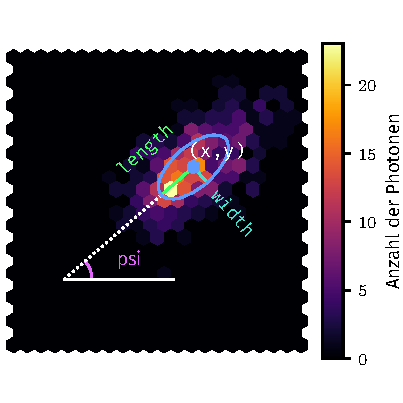
\includegraphics[width=0.5\textwidth]{Plots/hillas_2.pdf}
  \centering
  \caption{Schematische Darstellung der Hillasparameter, die das Kamerabild der Schauer charakterisieren. Diese Parameter
            werden verwendet, um die Energie des primären Teilchens zu schätzen.~\cite{Hillas_Max}}
  \label{abb:Hillas}
\end{figure}
Einen weiteren wichtigen Parameter bildet die totale Intensität des Bildes und da CTA aus mehreren unterschiedlichen Teleskopen besteht, bekommt die Anzahl
der Teleskope, die den gleichen Schauer gesehen haben, und welche Art von Teleskop dieses Schauer gesehen hat, eine große Bedeutung für die anschließende
Signal Separation und Energie Schätzung.
Diese Parameter werden genutzt um die Untergrundschauer von den photoninduzierten Schauern zu trennen.
Diese Aufgabe wird mit einer Klassifizierungsmethode des maschinellen Lernens gelöst.
%Durch das Verhältnis von Signal zu Untergrund von $\approx \frac{1}{1000}$~\cite{Cherenkov_Licht} wird eine große Menge Trainingsdaten
%benötigt, um eine gute Trennung zu ermöglichen.

Für die Schätzung der Photonenergie werden Regressionsmethoden verwendet, wobei der RF sich als stabilster Algorithmus erweist~\cite{Cherenkov_Licht}.
Die in \autoref{sec:ML} aufgeführten Annahmen für eine erfolgreiche Regressionsanalyse, sind bei diesem Problem bestmöglich erfüllt. Die Trainingsdaten
werden durch Monte Carlo Simulationen erstellt, die die Wechselwirkung der Primär- und Sekundärteilchen mit der Atmosphäre und die Reaktion des Teleskops
auf das Schauerlicht simuliert.
Dadurch repräsentiert der Trainingsdatensatz das Problem bestmöglich, jedoch führen mögliche systematische Fehler in der Simulation zu einer Verzerrung.
Darüber hinaus werden die Parameter mit der größtmöglichen Präzision gemessen, um den Fehler der Parameter zu minimieren,
jedoch sind aufgrund der Berechnung der Hillasparameter, welche in ~\cite[102]{HESS}
genauer beschrieben werden, diese nicht linear unabhängig.
Auch die Varianz des Fehlers geht aufgrund der unterschiedlichen Sensitivitäten der Teleskope nicht homogen
über den ganzen Energiebereich, was jedoch durch eine Gewichtung ausgeglichen werden könnte.

\section{Modellevaluation}
\label{sec:Per}

Um zu erkennen, ob das weiterentwickelte Modell eine genauere Vorhersage liefert als das Bisherige, muss die
Qualität des RFs beurteilt werden können.

Für einen ersten Überblick über die Genauigkeit des Algorithmus, wird die Wahrheit gegen die Vorhersage in einem
zweidimensionalen Histogramm aufgetragen, welches als Migrationsmatrix bezeichnet wird.
Dabei hat die Diagonale die Bedeutung der exakten Vorhersage und eine geringe Streuung der gefüllten Bins
um diese deutet auf einen guten Schätzer hin.
Die Aussagekraft dieser Abbildung hängt von der Anzahl der Bins ab, daher wird ein Raster von $300 \times 300$ verwendet.

Ein mögliches Maß, um die Anpassungsgüte von Regressionsmodellen beurteilen zu können, stellt der Determinationskoeffizient dar, welcher
durch
\begin{equation}
  R^2 = 1 - \frac{\sum_i (y_i-\hat{y}_i)^2}{\sum_i (y_i - \overline{y})^2}
\end{equation}
definiert wird. Wobei $\hat{y_i}$ die Schätzwerte, $\overline{y}$ der Mittelwert und $y_i$ die Messwerte darstellen.
Der Determinationskoeffizient nimmt den Wert $1$ an, wenn das Modell die Messpunkte exakt beschreibt und bei dem Wert $0$ ist
die Schätzung so gut wie die Verwendung des Mittelwerts als Schätzung. Wenn jedoch
$R^2 \leq 0$ ist, kann das Modell als unbrauchbar eingestuft werden, da die Attribute $X$ keine Information zur
Lösung des Problems einbringen.

Dieser Koeffizient besitzt Grenzen der Interpretierbarkeit, da er nur eine Aussage über das gesamte Modell macht und
nicht über die Genauigkeit in einzelnen Wertebereichen.
Außerdem reagiert er empfindlich gegenüber Trends, die $R^2$ senken, obwohl dies nicht bedeutet, dass das Modell die Abhängigkeiten des Problems
nicht gut beschreibt.
Des Weiteren muss die gleiche Anzahl an Datenpunkten vorliegen, um Modelle
miteinander zu vergleichen.

Eine Aussage über die Genauigkeit des Algorithmus kann auch über den relativen Fehler getroffen werden. Dabei spielen der Mittelwert und die
Hälfte des Interquartilen Abstandes (IQA) von $\SI{68.26}{\percent}$, der durch
\begin{equation}
  \operatorname{IQA} = \frac{Q_{84}-Q_{16}}{2}
\end{equation}
definiert wird, eine wichtige Rolle.
Dabei stellt $Q_{84}$ das $\SI{84.13}{\percent}$ Quantil und $Q_{15}$ das $\SI{15.87}{\percent}$ Quantil dar, welche durch die \textsc{numpy}-Bibliothek~\cite{scipy}
bestimmt werden, die das $q$-te Quantil als den $q \cdot N$-ten Wert eines geordneten Datensatzes der Größe $N$ definiert.
Der Mittelwert ist ein Maß für die Verzerrung und der $\operatorname{IQA}$ ist ein Maß für die Auflösung des Schätzers, wobei dies für unterschiedliche
Energie-Bins untersucht wird, da aufgrund der energieabhängigen Statistik auch diese Werte über das Energiespektrum hinweg variieren.

Ein weiteres Maß stellt der Mittlere quadratische Fehler
\begin{equation}
  \operatorname{mse} = \frac{1}{N} \sum_i (y_i-\hat{y}_i)^2
\end{equation}
dar.
Wenn dieser Fehler kleiner wird, verringert sich auch der relative Fehler, jedoch ist die Größe der Verringerung abhängig vom Energiebereich.
Wie in \autoref{sec:RF} beschrieben, wird der RF anhand dieses Kriteriums optimiert.

Die Frage ob der relative Fehler oder der $\operatorname{mse}$ minimiert werden soll, hängt von der angestrebten Analyse ab.
Soll ein Energiespektrum erstellt werden, um ein Potenzgesetz zu analysieren, bietet sich die Minimierung des relativen Fehlers an, da die
Energie logarithmisch aufgetragen wird.
Ist jedoch die Untersuchung eines Linienspektrums, wie bei der Suche nach Zerfällen der Dunklen Materie, die Absicht der Analyse, dann sollte
der absolute Fehler in dem zu analysierenden Energiebereich minimiert werden.


Um die Frage des Informationsgehalts der Attribute zu beantworten, kann zum Beispiel die Wichtigkeit mithilfe von Selektionshäufigkeit, Gini-Wichtigkeit oder
die Wichtigkeit der Permutations-Genauigkeit bestimmt werden.
Die in \textsc{scikit-learn} implementierte Methode nutzt die Rangordnung der Attribute in den einzelnen Entscheidungsbäumen, indem die früh und häufig genutzten Attribute
als wichtiger klassifiziert werden\cite{sklearn_FI}.
Diese Wichtigkeit kann für jeden Baum ausgelesen werden und als Boxplot dargestellt werden.
Dabei stellt die durchgezogene Linie den Median dar, die Enden des Kastens das $\num{0.25}$-und das $\num{0.75}$-Quartil, die Antennen das $\num{0.125}$-und das
$\num{0.875}$-Quantil und die Punkte stellen Ausreißer, die außerhalb des $\num{0.75}$-IQA liegen, dar.
Wenn eine unterschiedliche Zahl an Kategorien oder ein unterschiedlich großer Wertebereich der Attribute vorliegt, besitzt Bootstrapping mit Ersetzen der Datenpunkte
und die Attribut Selektion bei CART Algorithmen eine Verzerrung, welche sich auf die Bestimmungsmethoden der Wichtigkeit überträgt und somit das Ergebnis verfälschen
kann~\cite{feature_importance}.
